\documentclass[a4paper,12pt]{article}
\usepackage{geometry}
\geometry{a4paper, margin=1in}

\usepackage{amsmath}
\usepackage{amssymb}
\usepackage{graphicx}
\usepackage{float}
\usepackage[
    colorlinks=true,
    linkcolor=blue,
    citecolor=teal,
    urlcolor=blue
]{hyperref}
\usepackage{booktabs}
\usepackage{caption}
\usepackage[utf8]{inputenc}
\usepackage{subcaption}
\usepackage{colortbl}
\usepackage{xcolor}
\usepackage{ragged2e}
\usepackage{algorithm}
\usepackage{algpseudocode}
\usepackage{tikz}

\usepackage{array}
\usepackage[table]{xcolor}
\usetikzlibrary{shapes.geometric, arrows.meta, positioning, shadows, fit, calc}

\parindent 0px

% Custom Colors
\definecolor{myorange}{rgb}{0.85, 0.49, 0.13}
\definecolor{myblue}{rgb}{0.15, 0.65, 0.90}
\definecolor{mygreen}{rgb}{0.19, 0.82, 0.28}
\definecolor{myred}{rgb}{0.85, 0.11, 0.11}

\title{Deepfake Detection}
\author{ }
\date{\today}

\begin{document}

\begin{titlepage}
    \begin{center}
        \vspace*{1.2cm}
        {\Large \textbf{BANGLADESH UNIVERSITY OF ENGINEERING AND TECHNOLOGY}}
        
        \vspace{1.0cm}
        {\large \textbf{DEPARTMENT OF COMPUTER SCIENCE AND ENGINEERING}}
        \vspace{1.8cm}
        
        {\large \textbf{Course No:} CSE 200} \\[0.35cm]
        {\large \textbf{Course Title:} Technical Writing and Presentation}

        \vfill
        {\Large \textbf{A Report on}} \\[0.5cm]
        \rule{\linewidth}{0.6mm} \\[0.4cm]
        {\Huge \textbf{DEEPFAKE DETECTION}} \\[0.2cm]
        \rule{\linewidth}{0.6mm}
        \vfill
        {\large \today}
        \vfill
        \begin{minipage}{0.85\textwidth}
            \centering
            {\large \textbf{Subsection:}} C2 \qquad\qquad {\large \textbf{Group:}} 01 \\[0.35cm]
            \rule{0.67\textwidth}{0.3mm} \\[0.5cm]
            
            \begin{tabular}{r l}
                \textbf{Md. Mufeed Talukder}        & : 2305151 \\
                \textbf{Khandoker Md Tanjinul Islam} & : 2305159 \\
                \textbf{Md. Tahmidul Islam}         & : 2305180 \\
            \end{tabular}
        \end{minipage}

        \vspace*{1.5cm}
    \end{center}
\end{titlepage}

\tableofcontents

\newpage

\begin{center}
    \rule{\linewidth}{0.4mm} \\[1em]
    \textbf{\Large Deepfake Detection} \\
    \rule{\linewidth}{0.4mm}
\end{center}

\vspace{0.5cm}

\begin{center}
    \begin{large}
        \textbf{Abstract} \\[0.5cm]
    \end{large}
    \begin{minipage}{0.85\textwidth}
        \justify
        A deepfake is a synthetic image, video, or audio clip generated by deep neural networks to resemble a real person convincingly. Advances in autoencoder- and Generative Adversarial Network (GAN)-based architectures have made such media cheap to produce and difficult to distinguish from authentic recordings, creating a growing risk to journalism, elections, financial systems, and personal privacy. This report examines the deepfake problem from generation through detection to prevention. We first describe the encoder-decoder pipeline that produces synthetic media and the objective functions that drive it. We then present two complementary detection strategies: passive detection, which inspects spatial, temporal, and audio-visual artifacts left behind by the generation process, and proactive defense, which embeds cryptographic watermarks and provenance metadata at the point of creation so that origin can be verified later. We compare the two strategies, outline where each is used in practice, and argue that no single detector is a durable solution because detection and generation are locked in an adversarial cycle. We close by discussing the shift toward content provenance standards such as C2PA and the open challenges that remain.
    \end{minipage}
\end{center}

\vspace{0.5cm}

% =====================================================
\section{Introduction}
\label{sec:introduction}

A \textbf{deepfake} is a piece of synthetic media, typically an image, a video, or an audio clip, in which a deep neural network has replaced or altered a person's likeness so that the result appears authentic. The term is a portmanteau of ``deep learning'' and ``fake,'' and it reflects the underlying technique: a neural network learns the statistical structure of a person's face or voice from real examples and then uses that structure to generate new, fabricated content.

Deepfake technology is not inherently malicious. The same generative models are used for film dubbing, historical restoration, and accessibility tools. However, the ease with which convincing fake media can now be produced has created a genuine problem of trust. A fabricated speech by a public official, a cloned voice used to authorize a fraudulent wire transfer, or a manipulated video used to harass an individual are no longer hypothetical scenarios; each has already occurred. Because a single realistic fake can spread faster than a correction, the cost of being wrong about authenticity has grown substantially.

This report is organized around three questions that mirror the stages of the deepfake life cycle.
\begin{itemize}
    \item How is synthetic media generated? (Section~\ref{sec:generation})
    \item How can synthetic media be detected after it has been created? (Section~\ref{sec:detection})
    \item How can the origin of media be proven before it is ever questioned? (Section~\ref{sec:defense})
\end{itemize}
We conclude by comparing these approaches, listing domains where detection is already deployed, and outlining open challenges for the field (Sections~\ref{sec:applications}--\ref{sec:conclusion}).

% =====================================================
\section{Generation of Deepfake Media}
\label{sec:generation}

Before detection can be discussed meaningfully, we must understand what a detector is looking for. This section describes the general architecture used to generate face- and voice-based deepfakes and the mathematical objective that drives training.

\subsection{General Architecture}
\label{subsec:gen-architecture}

Most face-swapping and face-reenactment systems share a common structure, illustrated in Figure~\ref{fig:gen-architecture}. Two inputs are required: a \textit{source identity}, which supplies the face or voice to be inserted, and a \textit{target context}, which supplies the video or audio in which that identity should appear. Both inputs are passed to a deep learning engine, most commonly an autoencoder or a Generative Adversarial Network (GAN), which encodes each input into a compact latent representation and then decodes that representation into a synthetic output that combines the identity of the source with the motion, lighting, and background of the target.

\begin{figure}[H]
    \centering
    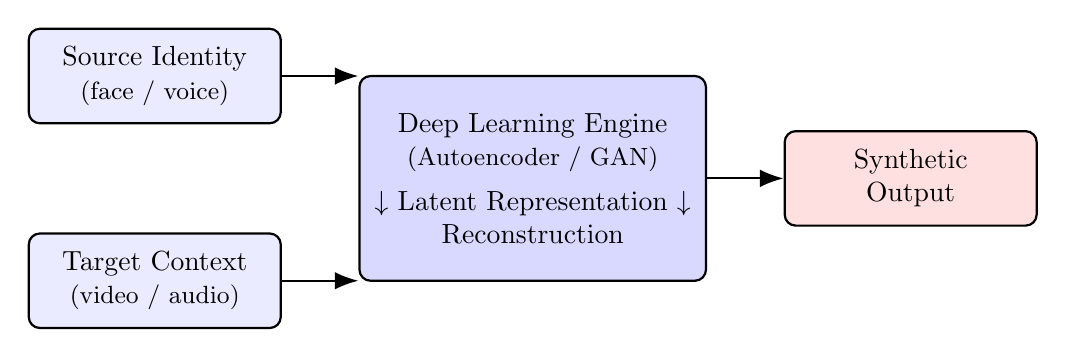
\begin{tikzpicture}[
        imgbox/.style={rectangle, rounded corners, draw, thick, fill=blue!8, minimum width=3.2cm, minimum height=1.2cm, align=center},
        net/.style={rectangle, rounded corners, draw, thick, fill=blue!15, minimum width=4.4cm, minimum height=2.6cm, align=center},
        outbox/.style={rectangle, rounded corners, draw, thick, fill=red!12, minimum width=3.2cm, minimum height=1.2cm, align=center},
        arrowline/.style={-{Latex[length=3mm]}, thick}
    ]
        \node[imgbox] (src) at (0,1.3) {Source Identity\\ \small (face / voice)};
        \node[imgbox] (tgt) at (0,-1.3) {Target Context\\ \small (video / audio)};
        \node[net] (engine) at (4.8,0) {Deep Learning Engine\\ \small (Autoencoder / GAN)\\[0.15cm] $\downarrow$ Latent Representation $\downarrow$\\ Reconstruction};
        \node[outbox] (out) at (9.6,0) {Synthetic\\Output};
        \draw[arrowline] (src.east) -- (engine.west |- src.east);
        \draw[arrowline] (tgt.east) -- (engine.west |- tgt.east);
        \draw[arrowline] (engine.east) -- (out.west);
    \end{tikzpicture}
    \caption{General deepfake generation pipeline. A source identity and a target context are encoded into a shared latent space and decoded into a synthetic output.}
    \label{fig:gen-architecture}
\end{figure}

\subsection{Mathematical Formulation}
\label{subsec:gen-math}

Let $x$ denote an input image, video frame, or audio segment drawn from a training dataset $\mathcal{D}$. An autoencoder-based generator consists of an encoder $E_\phi$ and a decoder $G_\theta$, where $\phi$ and $\theta$ are learned parameters. The encoder maps the input to a latent vector $z = E_\phi(x)$, and the decoder reconstructs an output $\hat{x} = G_\theta(z)$. Training minimizes the reconstruction loss
\begin{equation}
    \mathcal{L}_{\text{recon}} = \mathbb{E}_{x \sim \mathcal{D}} \left[ \lVert x - \hat{x} \rVert_2^2 \right],
    \label{eq:recon-loss}
\end{equation}
where $\lVert \cdot \rVert_2$ denotes the Euclidean norm. A face-swapping system typically trains one shared encoder alongside two separate decoders, one for each identity, so that a face encoded from person A can be decoded through person B's decoder to produce a face that has A's expression and B's identity.

Many modern generators improve realism further by pairing the decoder $G_\theta$ with a discriminator $D_\psi$, forming a Generative Adversarial Network. The discriminator is trained to distinguish real data from generated data, while the generator is trained to fool the discriminator. This adversarial relationship is expressed as the minimax objective
\begin{equation}
    \min_{\theta} \max_{\psi} \; V(D_\psi, G_\theta) = \mathbb{E}_{x \sim \mathcal{D}} \left[ \log D_\psi(x) \right] + \mathbb{E}_{z \sim p(z)} \left[ \log \left( 1 - D_\psi(G_\theta(z)) \right) \right],
    \label{eq:gan-loss}
\end{equation}
where $p(z)$ is a prior distribution, often Gaussian, from which latent vectors are sampled. As training proceeds, $D_\psi$ becomes better at spotting fakes, which in turn forces $G_\theta$ to produce increasingly realistic output; this adversarial pressure is precisely what makes GAN-based deepfakes difficult to detect by eye. It is also the same adversarial pattern, generator against discriminator, that reappears later at the level of the entire field, where a detector plays the role of $D_\psi$ and a new generation technique plays the role of $G_\theta$ (Section~\ref{subsec:cat-mouse}).

\subsection{Illustrative Example}
\label{subsec:gen-example}

Figure~\ref{fig:gen-example} shows a single face-swap example that follows the pipeline of Figure~\ref{fig:gen-architecture}: a source image supplies the identity, a target image supplies the pose and background, and the outcome is a synthetic frame in which the source identity has been transferred onto the target context. The example reused from our presentation slides is suitable for this figure; no new image is required here.

\begin{figure}[H]
    \centering
    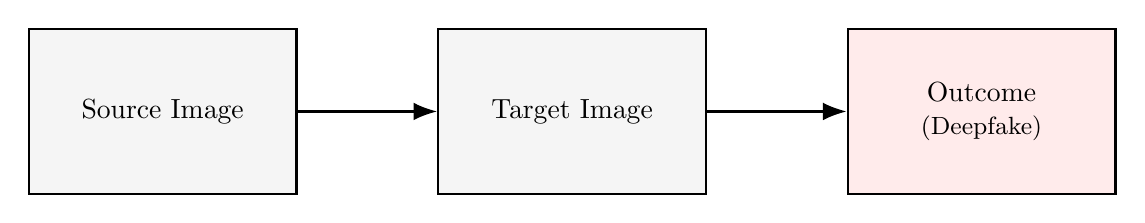
\begin{tikzpicture}[
        ph/.style={rectangle, draw, thick, fill=gray!8, minimum width=3.4cm, minimum height=2.1cm, align=center},
        arrowline/.style={-{Latex[length=3mm]}, thick}
    ]
        % \node[ph] (s) at (0,0) {\includegraphics[width=3.1cm]{report_images/example_source.png}};
        \node[ph] (s) at (0,0) {Source Image};
        % \node[ph] (t) at (5.2,0) {\includegraphics[width=3.1cm]{report_images/example_target.png}};
        \node[ph] (t) at (5.2,0) {Target Image};
        % \node[ph, fill=red!8] (o) at (10.4,0) {\includegraphics[width=3.1cm]{report_images/example_output.png}};
        \node[ph, fill=red!8] (o) at (10.4,0) {Outcome\\ \small (Deepfake)};
        \draw[arrowline] (s.east) -- (t.west);
        \draw[arrowline] (t.east) -- (o.west);
    \end{tikzpicture}
    \caption{Source, target, and outcome for a single face-swap example (reuse \texttt{example\_source}, \texttt{example\_target}, \texttt{example\_output} from the presentation).}
    \label{fig:gen-example}
\end{figure}

% =====================================================
\section{Passive Detection: Finding the Flaws}
\label{sec:detection}

Detection strategies fall into two broad categories, summarized in Table~\ref{tab:passive-proactive}: \textit{passive detection}, which examines media after it has been created, and \textit{proactive defense}, which embeds safeguards into the generation process itself. This section covers passive detection; proactive defense is discussed in Section~\ref{sec:defense}.

\begin{table}[H]
    \centering
    \renewcommand{\arraystretch}{1.3}
    \begin{tabular}{@{} >{\raggedright\arraybackslash}p{3.2cm} >{\raggedright\arraybackslash}p{5.6cm} >{\raggedright\arraybackslash}p{5.6cm} @{}}
        \toprule
        \rowcolor{gray!15}
        \textbf{Aspect} & \textbf{Passive Detection} & \textbf{Proactive Defense} \\
        \midrule
        \hline
        \textbf{When it acts} & After media has been created & At the moment media is created \\
        \hline
        \textbf{Method} & Examines media for hidden artifacts left by the generation process & Embeds a cryptographic watermark or provenance record into the media \\
        \hline
        \textbf{Posture} & Reactive & Preventative \\
        \hline
        \textbf{Typical question} & \textit{``Does this look fake?''} & \textit{``Can we prove where this came from?''} \\
        \bottomrule
    \end{tabular}
    \caption{Comparison of passive detection and proactive defense.}
    \label{tab:passive-proactive}
\end{table}

\subsection{Spatial Artifact Detection}
\label{subsec:spatial}

A single frame is often enough to reveal a deepfake. Generative models tend to leave two characteristic spatial artifacts. First, skin regions are frequently over-smoothed because the decoder averages over many training examples, producing a waxy texture that lacks natural pore-level detail. Second, generated faces often exhibit an unnaturally even focus: the face and the background are equally sharp, whereas a real photograph taken with a camera lens shows a shallow depth of field that blurs the background relative to the subject.

These cues can be learned automatically. A Convolutional Neural Network (CNN) is trained as a binary classifier $f_w : x \mapsto p \in [0,1]$, where $x$ is an input frame, $w$ denotes the network's weights, and $p$ is the predicted probability that the frame is synthetic. Given a labeled training set of real and fake frames with ground-truth labels $y \in \{0, 1\}$, the network is trained by minimizing the binary cross-entropy loss
\begin{equation}
    \mathcal{L}_{\text{BCE}} = -\frac{1}{N} \sum_{i=1}^{N} \left[ y_i \log(p_i) + (1 - y_i) \log(1 - p_i) \right],
    \label{eq:bce-loss}
\end{equation}
where $N$ is the number of training examples in a mini-batch. Figure~\ref{fig:spatial} illustrates the two artifacts described above together with the classification pipeline.

\begin{figure}[H]
    \centering
    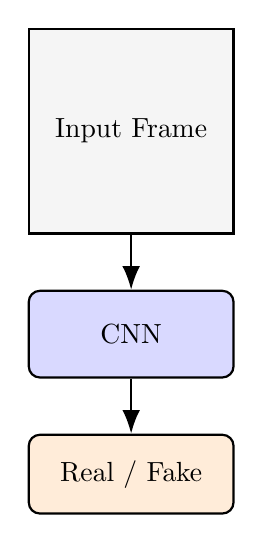
\begin{tikzpicture}[
        node distance=0.7cm,
        net/.style={rectangle, rounded corners, draw, thick, minimum width=2.6cm, minimum height=1.1cm, fill=blue!15, align=center},
        outbox/.style={rectangle, rounded corners, draw, thick, minimum width=2.6cm, minimum height=1cm, fill=orange!15, align=center},
        arrowline/.style={-{Latex[length=3mm]}, thick}
    ]
        \node[draw, thick, minimum width=2.6cm, minimum height=2.6cm, fill=gray!8] (frame) {Input Frame};
        \node[net, below=of frame] (cnn) {CNN};
        \node[outbox, below=of cnn] (out) {Real / Fake};
        \draw[arrowline] (frame) -- (cnn);
        \draw[arrowline] (cnn) -- (out);
    \end{tikzpicture}
    \caption{A CNN classifier trained to distinguish real frames from synthetic ones using spatial cues such as skin smoothness and depth-of-field consistency.}
    \label{fig:spatial}
\end{figure}

\subsection{Temporal Artifact Detection}
\label{subsec:temporal}

A single frame can look convincing while the video as a whole does not, because generative models operate mostly on a frame-by-frame basis and are not always consistent across time. Three temporal cues are commonly exploited.
\begin{itemize}
    \item \textbf{Blink rate:} humans blink at a fairly regular interval; early face-swap datasets under-represented closed-eye frames, causing generated subjects to blink too rarely or too regularly.
    \item \textbf{Motion smoothness:} synthetic faces can exhibit subtle jitter or warping between consecutive frames that a real camera recording would not produce.
    \item \textbf{Physiological signal:} a real face shows faint, periodic color shifts caused by blood flow beneath the skin (remote photoplethysmography); this signal is difficult for a generator to reproduce consistently.
\end{itemize}
Because these cues depend on the relationship between frames rather than on any single frame, they are best captured by a sequence model such as a Long Short-Term Memory (LSTM) network or a Vision Transformer applied across a short clip $\{x_1, x_2, \dots, x_T\}$, where $T$ is the number of frames in the clip. The sequence model is trained with the same binary cross-entropy objective as Equation~\ref{eq:bce-loss}, but the input is now a temporal window rather than a single frame.

\subsection{Multimodal Detection}
\label{subsec:multimodal}

Voice can be cloned just as convincingly as a face can be swapped, and an attacker who fakes only one modality often leaves the other unchanged, which creates an inconsistency that can be measured directly. The most reliable cue in this category is lip-sync mismatch: the shape of the mouth in the video should match the phoneme being produced in the audio at every instant, and a mismatch of even a few frames is detectable even when neither the video nor the audio is individually flagged as fake by a single-modality detector.

A multimodal detector processes the video stream and the audio stream separately, using a video encoder for the former and an audio encoder in the style of Whisper or wav2vec2 for the latter, and then combines the two streams with a cross-modal transformer that checks whether the acoustic and visual signals are consistent with each other. This cross-checking approach is powerful precisely because it does not require either modality to be individually recognizable as synthetic; it only requires the two to disagree.

\subsection{The Cat-and-Mouse Problem}
\label{subsec:cat-mouse}

Passive detection faces a structural limitation. Every new detection technique that becomes public gives generator designers a specific artifact to correct in the next model version, so detection accuracy that is measured on today's fakes routinely degrades on tomorrow's. This dynamic mirrors the adversarial training objective of Equation~\ref{eq:gan-loss} at the scale of the research community: detectors act as an external discriminator, and generators are iteratively improved to defeat them. Because detection is always one step behind the latest generation technique, passive detection alone cannot be a permanent solution; it must be paired with a proactive strategy, which we discuss next.

% =====================================================
\section{Proactive Defense: Proving Provenance}
\label{sec:defense}

Rather than trying to spot a fake after it exists, a proactive defense makes authenticity verifiable from the moment media is created.

\subsection{Invisible Watermarking}
\label{subsec:watermark}

An invisible watermark is a pattern embedded directly into a generated image or video at creation time, using a cryptographic key $k$ known to the issuing organization. The watermark embedding function can be described as $x_w = W_k(x)$, where $x$ is the generator's raw output, $x_w$ is the watermarked output, and $W_k$ is the embedding operator. The pattern is designed to be perceptually invisible, so $x_w$ and $x$ look identical to a human viewer, while remaining statistically detectable to a verification system that has access to the key. A well-designed watermark is also robust: it should survive common transformations such as compression, cropping, and re-encoding through a screenshot, so that the provenance signal is not lost as content is shared across platforms.

Verification is the mirror operation of embedding: given a piece of media and the same key $k$, a verification system extracts a candidate pattern and checks it for a match. Figure~\ref{fig:watermark} summarizes the pipeline from generation through verification.

\begin{figure}[H]
    \centering
    \resizebox{\textwidth}{!}{%
    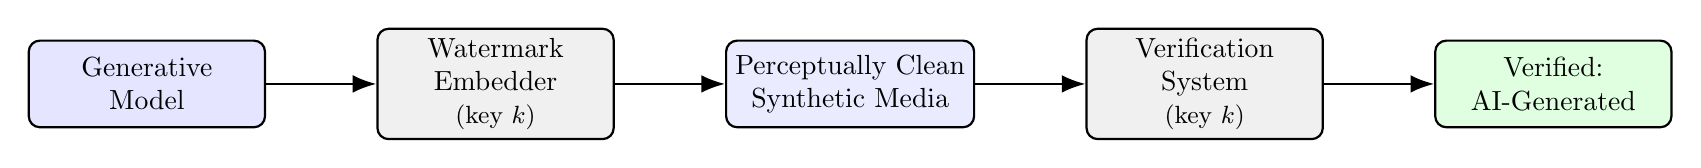
\begin{tikzpicture}[
        node distance=1.0cm and 1.4cm,
        box/.style={rectangle, rounded corners, draw, thick, minimum width=3cm, minimum height=1.1cm, align=center},
        arrowline/.style={-{Latex[length=3mm]}, thick}
    ]
        \node[box, fill=blue!10] (gen) {Generative\\Model};
        \node[box, right=of gen, fill=gray!12] (embed) {Watermark\\Embedder \\ \small (key $k$)};
        \node[box, right=of embed, fill=blue!8] (media) {Perceptually Clean\\Synthetic Media};
        \node[box, right=of media, fill=gray!12] (verify) {Verification\\System \\ \small (key $k$)};
        \node[box, right=of verify, fill=green!12] (result) {Verified:\\AI-Generated};
        \draw[arrowline] (gen) -- (embed);
        \draw[arrowline] (embed) -- (media);
        \draw[arrowline] (media) -- (verify);
        \draw[arrowline] (verify) -- (result);
    \end{tikzpicture}%
    }
    \caption{Invisible watermarking pipeline: a key-dependent pattern is embedded at generation time and later extracted by a verification system.}
    \label{fig:watermark}
\end{figure}

\subsubsection*{Watermarking in Action}
As a concrete industrial deployment of generation-time watermarking, Anthropic's Claude models offer an illustrative example. 
Anthropic's implementation is a version of SynthID-Text, the method Google DeepMind published in Nature in 2024 and deployed on Gemini, 
demonstrating the convergence of independent AI developers on a shared watermarking paradigm \cite{dathathri2024scalable}.

The mechanism operates at the token-sampling stage rather than as a post-hoc transformation of the output. 
During autoregressive generation, a language model frequently faces multiple plausible continuations at a given 
position (e.g., completing "The sky was" with either "grey" or "cloudy"). In an unwatermarked system, ties among such 
near-equivalent candidates are resolved via an ordinary pseudorandom number generator. Anthropic's watermarking system 
instead uses a secret cryptographic key combined with information from the preceding tokens to influence this selection, 
biasing an otherwise-arbitrary choice according to a hidden, deterministic function of the key and local context.

Critically, this approach preserves output fidelity: every word in a watermarked output remains a word the model could have 
produced anyway, with nothing added to the text and no hidden characters inserted. Detectability is therefore statistical 
rather than lexical — no individual sentence appears unusual, and the signal exists only in aggregate across a sufficiently 
long span of text, requiring roughly 150–200 words for reliable detection. A party holding the key can, in principle, measure 
agreement between the observed token choices and those the keyed process would have generated, yielding a probabilistic estimate 
of authorship, while the pattern remains statistically invisible to any party lacking the key.


This case illustrates a central trade-off in text watermarking research: robustness to copy-paste propagation and imperceptibility 
to human readers, at the cost of detection reliability on short passages.
\subsection{Content Provenance Standards}
\label{subsec:c2pa}

Watermarking answers a narrow question: was this specific pattern present? A broader approach, known as content provenance, attaches a signed record of an asset's history, its origin, its creator, and every edit it has undergone, directly to the file as metadata. The Coalition for Content Provenance and Authenticity (C2PA) is the leading industry standard in this space; it defines \textit{Content Credentials} that travel with a media file and can be inspected by any compliant viewer. Table~\ref{tab:detection-vs-provenance} contrasts this provenance-based approach with the detection-based approach of Section~\ref{sec:detection}.

\begin{table}[H]
    \centering
    \renewcommand{\arraystretch}{1.3}
    \begin{tabular}{@{} >{\raggedright\arraybackslash}p{3.5cm} >{\raggedright\arraybackslash}p{6.0cm} >{\raggedright\arraybackslash}p{6.0cm} @{}}
        \toprule
        \rowcolor{gray!15}
        \textbf{Aspect} & \textbf{Detection} & \textbf{Provenance} \\
        \midrule
        \textbf{Question asked} & Does this look fake? & Can we prove where this came from? \\
        \midrule
        \textbf{Basis} & Statistical inference over artifacts & Cryptographic signature and metadata \\
        \midrule
        \textbf{Confidence} & Probabilistic; can be wrong & Deterministic, if the signature is intact \\
        \midrule
        \textbf{Weakness} & Loses ground as generators improve & Requires adoption across creation tools and platforms \\
        \bottomrule
    \end{tabular}
    \caption{Detection asks whether content looks fake; provenance asks whether its origin can be proven.}
    \label{tab:detection-vs-provenance}
\end{table}

% =====================================================
\section{Applications and Defense in Depth}
\label{sec:applications}

\subsection{Where Detection Matters}
\label{subsec:where}

The guarantees required of a detection system differ sharply by domain, as summarized in Table~\ref{tab:applications}.

\begin{table}[H]
    \centering
    \renewcommand{\arraystretch}{1.3}
    \begin{tabular}{@{} >{\raggedright\arraybackslash}p{3.6cm} >{\raggedright\arraybackslash}p{5.5cm} >{\raggedright\arraybackslash}p{5.5cm} @{}}
        \toprule
        \rowcolor{gray!15}
        \textbf{Domain} & \textbf{Typical Use} & \textbf{Primary Requirement} \\
        \midrule
        Social platforms & Upload scanning, content labeling & High throughput, low latency \\
        \midrule
        FinTech and identity & Fraud prevention, liveness checks & Low false-negative rate \\
        \midrule
        Courts and forensics & Evidence auditing, forensic verification & High explainability, legal defensibility \\
        \midrule
        Government and elections & Statement verification, media integrity & Public trust, rapid response \\
        \bottomrule
    \end{tabular}
    \caption{Representative application domains for deepfake detection and their primary requirements.}
    \label{tab:applications}
\end{table}

\subsection{Defense in Depth}
\label{subsec:defense-in-depth}

No single technique from Sections~\ref{sec:detection} and~\ref{sec:defense} is sufficient on its own. In practice, an effective system layers three stages, illustrated in Figure~\ref{fig:defense-in-depth}: \textit{prevention}, which limits access to generation tools and embeds watermarks; \textit{detection}, which screens content already in circulation using spatial, temporal, and audio-visual cues; and \textit{verification}, which checks cryptographic provenance when it is available. Each stage compensates for the weaknesses of the others, so that a failure at one stage does not compromise the whole system.

\begin{figure}[H]
    \centering
    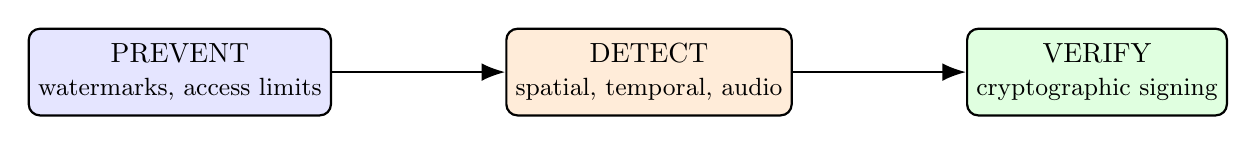
\begin{tikzpicture}[
        node distance=2.2cm,
        box/.style={rectangle, rounded corners, draw, thick, minimum width=3cm, minimum height=1.1cm, align=center},
        arrowline/.style={-{Latex[length=3mm]}, thick}
    ]
        \node[box, fill=blue!10] (prevent) {PREVENT\\\small watermarks, access limits};
        \node[box, right=of prevent, fill=orange!15] (detect) {DETECT\\\small spatial, temporal, audio};
        \node[box, right=of detect, fill=green!12] (verify) {VERIFY\\\small cryptographic signing};
        \draw[arrowline] (prevent) -- (detect);
        \draw[arrowline] (detect) -- (verify);
    \end{tikzpicture}
    \caption{Defense in depth: prevention, detection, and verification act as three complementary layers rather than a single point of failure.}
    \label{fig:defense-in-depth}
\end{figure}

Algorithm~\ref{alg:pipeline} summarizes the operational logic of a layered detection service that combines a passive classifier with provenance verification.

\begin{algorithm}[H]
\caption{Layered Screening of an Uploaded Media Item}
\label{alg:pipeline}
\begin{algorithmic}[1]
\Require Media item $x$, watermark key $k$, spatial detector $f_w$, temporal detector $g_v$, decision threshold $\tau$
\State Attempt to extract a provenance record or watermark from $x$ using key $k$
\If{a valid, matching record is found}
    \State \Return \textsc{Verified Authentic}
\Else
    \State Compute spatial score $p_s \gets f_w(x)$ (Equation~\ref{eq:bce-loss})
    \State Compute temporal score $p_t \gets g_v(x)$ over a short clip
    \State Combine scores: $p \gets \tfrac{1}{2}(p_s + p_t)$
    \If{$p > \tau$}
        \State \Return \textsc{Flagged as Likely Synthetic}
    \Else
        \State \Return \textsc{Passed, No Provenance Record}
    \EndIf
\EndIf
\end{algorithmic}
\end{algorithm}

% =====================================================
\section{Challenges and Future Directions}
\label{sec:challenges}

Sections~\ref{sec:detection} and~\ref{sec:defense} show what passive detection and proactive provenance can do under controlled conditions; three difficulties determine whether they hold up in deployment. First, detectors generalize poorly across generators: a systematic review of cross-dataset benchmarks found accuracy declines of roughly 11\% for transformer-based detectors and over 15\% for CNN-based detectors when tested against an unseen generator family \cite{raza2026review}, and the field's response is domain-generalized and meta-learning detectors trained to be invariant to generator identity rather than tuned to one \cite{nguyenle2026survey}. Second, a detector or a watermark can be evaded deliberately rather than merely outdated: small, imperceptible perturbations have been shown to flip a detector's decision or strip an embedded watermark, and such attacks transfer across schemes the adversary never directly queried \cite{jiang2023evading}. Third, the trust infrastructure behind provenance is itself imperfect: an independent 2026 security analysis found the C2PA specification incomplete and open to forgery in places, with one hardware vendor forced to revoke every content credential it had issued after a signing flaw \cite{golaszewski2026c2pa} -- even as the European Union's AI Act now legally requires this kind of provenance marking, with Article~50 obligations in force from 2~August~2026 and fines of up to 3\% of global turnover \cite{euaiact2024}. Table~\ref{tab:challenges} summarizes these challenges alongside the field's response.

\begin{table}[H]
    \centering
    \renewcommand{\arraystretch}{1.5}
    \begin{tabular}{|p{4.4cm}|p{5.8cm}|p{4.0cm}|}
        \hline
        \textbf{Challenge} & \textbf{Evidence} & \textbf{Response} \\ \hline
        Poor cross-generator generalization & Cross-dataset AUC drops $\sim$11\% (transformer) to $>$15\% (CNN) \cite{raza2026review} & Domain-generalized, meta-learning detectors \cite{nguyenle2026survey} \\ \hline
        Adversarial evasion of detectors/watermarks & Imperceptible perturbations flip decisions or strip watermarks \cite{jiang2023evading} & Adversarially hardened detectors and watermarks \\ \hline
        Gaps in provenance trust infrastructure & C2PA found incomplete; credential revocations have occurred \cite{golaszewski2026c2pa} & Independent audits, stronger CA infrastructure \\ \hline
        Regulation outpacing technical readiness & EU AI Act Article~50 mandates marking from Aug.\ 2026 \cite{euaiact2024} & Standardized provenance with detection as fallback \\ \hline
        Risk of full automation & Legal/ethical risk without human review (Section~\ref{subsec:where}) & Human-in-the-loop review \\ \hline
    \end{tabular}
    \caption{Key challenges in deepfake detection and the corresponding direction of response.}
    \label{tab:challenges}
\end{table}

These directions converge on the same picture: detection that is multimodal and generator-agnostic rather than tuned to one architecture, provenance that is independently audited rather than merely deployed, and human judgment retained for consequential decisions.

% =====================================================
\section{Conclusion}
\label{sec:conclusion}

Deepfake generation and detection are two sides of the same adversarial process described by Equation~\ref{eq:gan-loss}: as generators improve, detectors must improve to match them, and the cycle repeats. Passive detection, whether based on spatial artifacts (Section~\ref{subsec:spatial}), temporal inconsistency (Section~\ref{subsec:temporal}), or cross-modal mismatch (Section~\ref{subsec:multimodal}), remains useful but cannot win this race alone: it always responds to a technique that already exists, and, as Section~\ref{sec:challenges} showed, its accuracy transfers only partially from one generator to the next. Proactive defense through watermarking and content provenance (Section~\ref{sec:defense}) reframes the question from ``does this look fake?'' to ``can we prove where this came from?'', which is what makes verification durable as generation techniques advance -- though neither a detector nor a watermark is beyond deliberate evasion, and even the provenance standards meant to anchor this side still carry documented security gaps.

The goal, then, is not a perfect detector; no fixed classifier stays accurate indefinitely against a generator, or an adversary, built specifically to defeat it. The realistic goal is a layered ecosystem combining prevention, detection, and verification (Section~\ref{subsec:defense-in-depth}), each independently audited and continuously updated, so that fabricated media is harder to spread convincingly and genuine media is easier to verify. With the EU AI Act now requiring machine-readable marking of synthetic content \cite{euaiact2024}, this shift is no longer only academic: provenance infrastructure that was optional at the start of this report is fast becoming a legal expectation. As the technology and its governance mature together, we expect the balance to keep shifting from after-the-fact detective work toward built-in, verifiable authenticity.
\newpage
% =====================================================
% TO KEEP OR NOT TO KEEP THAT IS THE QUESTION
\nocite{goodfellow2014,rossler2019,li2020,agarwal2020,c2pa}
\bibliographystyle{plain}
\bibliography{Deepfake_Detection_Report}

\end{document}
